\chapter*{Dodatak: Prikaz aktivnosti grupe}
		\addcontentsline{toc}{chapter}{Dodatak: Prikaz aktivnosti grupe}
		
		\section*{Dnevnik sastajanja}
		
		%\textbf{\textit{Kontinuirano osvježavanje}}\\
		
		 %\textit{U ovom dijelu potrebno je redovito osvježavati dnevnik sastajanja prema predlošku.}
		
		\begin{packed_enum}
			\item  sastanak
			
			\item[] \begin{packed_item}
				\item Datum: 19. listopada 2023.
				\item Prisustvovali: D.Barukčić, L.Barić, N.Božić, K.Đunđek, L.Jukić, E.Samaržija, T.Topolovec
				\item Teme sastanka:
				\begin{packed_item}
					\item  upoznavanje
					\item  diskusija na temu projekta 
				\end{packed_item}
			\end{packed_item}
			
			\item  sastanak
			\item[] \begin{packed_item}
				\item Datum: 20. listopada 2023.
				\item Prisustvovali: D.Barukčić, L.Barić, N.Božić, K.Đunđek, L.Jukić, E.Samaržija, T.Topolovec
				\item Teme sastanka:
				\begin{packed_item}
					\item  podjela poslova i grupiranje unutarnjih timova 
					\item  dogovaranje oko tehnologija koje će se koristiti u izradi projekta
				\end{packed_item}
			\end{packed_item}
			
			\item  sastanak
			\item[] \begin{packed_item}
				\item Datum: 26. listopada 2023.
				\item Prisustvovali: D.Barukčić, L.Barić, N.Božić, K.Đunđek, L.Jukić, E.Samaržija, T.Topolovec
				\item Teme sastanka:
				\begin{packed_item}
					\item  razrada backenda 
					\item  ideje o izgledu stranice
					
				\end{packed_item}
			\end{packed_item}
			
			\item  sastanak
			\item[] \begin{packed_item}
				\item Datum: 3. studenoga 2023.
				\item Prisustvovali: D.Barukčić, L.Barić, N.Božić, K.Đunđek, L.Jukić, E.Samaržija, T.Topolovec
				\item Teme sastanka:
				\begin{packed_item}
					\item  izrada stranice, homepagea, logina i registracije
					\item  testiranje backenda
				\end{packed_item}
			\end{packed_item}
			
			\item  sastanak
			\item[] \begin{packed_item}
				\item Datum: 15. studenoga 2023.
				\item Prisustvovali: D.Barukčić, L.Barić, N.Božić, K.Đunđek, L.Jukić, E.Samaržija, T.Topolovec
				\item Teme sastanka:
				\begin{packed_item}
					\item  rasprava o deployu
					\item  završavanje dokumentacije
					\item  problemi u backendu 
				\end{packed_item}
			\end{packed_item}
			
			\item  sastanak
			\item[] \begin{packed_item}
				\item Datum: 21. prosinac 2023.
				\item Prisustvovali: D.Barukčić, L.Barić, N.Božić, K.Đunđek, L.Jukić, E.Samaržija, T.Topolovec
				\item Teme sastanka:
				\begin{packed_item}
					\item  podjela poslova
					\item  završetak backenda
					\item  ozbiljniji rad na frontendu
				\end{packed_item}
			\end{packed_item}
			
			\item  sastanak
			\item[] \begin{packed_item}
				\item Datum: 7. siječnja 2024.
				\item Prisustvovali: D.Barukčić, L.Barić, N.Božić, K.Đunđek, L.Jukić, E.Samaržija, T.Topolovec
				\item Teme sastanka:
				\begin{packed_item}
					\item  završna podjela poslova
					\item  dovrsšavanje dokumentacije
					\item  završetak frontenda
				\end{packed_item}
			\end{packed_item}
			
			%
			
		\end{packed_enum}
		
		\eject
		\section*{Tablica aktivnosti}
		
			%\textbf{\textit{Kontinuirano osvježavanje}}\\
			
			 %\textit{Napomena: Doprinose u aktivnostima treba navesti u satima po članovima grupe po aktivnosti.}

			\begin{longtblr}[
					label=none,
				]{
					vlines,hlines,
					width = \textwidth,
					colspec={X[7, l]X[1, c]X[1, c]X[1, c]X[1, c]X[1, c]X[1, c]X[1, c]}, 
					vline{1} = {1}{text=\clap{}},
					hline{1} = {1}{text=\clap{}},
					rowhead = 1,
				} 
				
				\SetCell[c=1]{c}{} & \SetCell[c=1]{c}{\rotatebox{90}{\textbf{Dominik Barukčić }}} & \SetCell[c=1]{c}{\rotatebox{90}{\textbf{Lana Barić }}} &	\SetCell[c=1]{c}{\rotatebox{90}{\textbf{Nika Božić }}} & \SetCell[c=1]{c}{\rotatebox{90}{\textbf{Kristina Đunđek }}} &	\SetCell[c=1]{c}{\rotatebox{90}{\textbf{Lovro Jukić }}} & \SetCell[c=1]{c}{\rotatebox{90}{\textbf{Ena Samaržija }}} &	\SetCell[c=1]{c}{\rotatebox{90}{\textbf{Tea Topolovec }}} \\  
				Upravljanje projektom               & 15 & 0 & 0 & 0 & 0 & 0 & 0 \\
				Opis projektnog zadatka            & 1  & 0 & 2 & 0 & 0 & 0 & 0 \\
				Funkcionalni zahtjevi              & 1  & 0 & 4 & 0 & 5 & 5 & 0 \\
				Opis pojedinih obrazaca            & 1  & 0 & 3 & 0 & 3 & 1 & 0 \\
				Dijagram obrazaca                  & 0  & 0 & 0 & 2 & 0 & 3 & 0 \\
				Sekvencijski dijagrami            & 0  & 2 & 0 & 3 & 0 & 0 & 0 \\
				Opis ostalih zahtjeva              & 0  & 3 & 0 & 0 & 0 & 0 & 0 \\
				Arhitektura i dizajn sustava       & 0  & 0 & 0 & 0 & 0 & 0 & 3 \\
				Baza podataka                      & 0  & 0 & 0 & 0 & 0 & 0 & 4 \\
				Dijagram razreda                   & 0  & 2 & 0 & 2 & 0 & 0 & 0 \\
				Dijagram stanja                    & 0  & 0 & 0 & 0 & 0 & 0 & 0 \\
				Dijagram aktivnosti                & 0  & 0 & 0 & 0 & 0 & 0 & 0 \\
				Dijagram komponenti                & 2  & 0 & 0 & 0 & 0 & 0 & 0 \\
				Korištene tehnologije i alati      & 1  & 0 & 0 & 0 & 0 & 0 & 0 \\
				Ispitivanje programskog rješenja   & 0  & 0 & 0 & 0 & 0 & 0 & 0 \\
				Dijagram razmještaja               & 1  & 0 & 0 & 0 & 0 & 0 & 0 \\
				Upute za puštanje u pogon          & 2  & 0 & 0 & 0 & 0 & 0 & 0 \\
				Dnevnik sastajanja                & 1  & 0 & 0 & 0 & 0 & 0 & 0 \\
				Zaključak i budući rad            & 2  & 0 & 0 & 0 & 0 & 0 & 0 \\
				Popis literature                  & 1  & 0 & 0 & 0 & 0 & 0 & 0 \\
				\textit{izrada baze podataka} 		 			& 0 & 0 & 0 & 0 & 0 & 0 & 4 \\  
				\textit{back end} 							& 0 & 13 & 0 & 14 & 0 & 0 & 11 \\  
				\textit{front end} 							& 0 & 13 & 0 & 14 & 0 & 0 & 11 \\  
				\textit{deploy} 							& 20 & 0 & 0 & 0 & 0 & 0 & 0 \\ 
			\end{longtblr}
					
					
		\eject
		\section*{Dijagrami pregleda promjena}
		
		 \begin{figure}[H]
			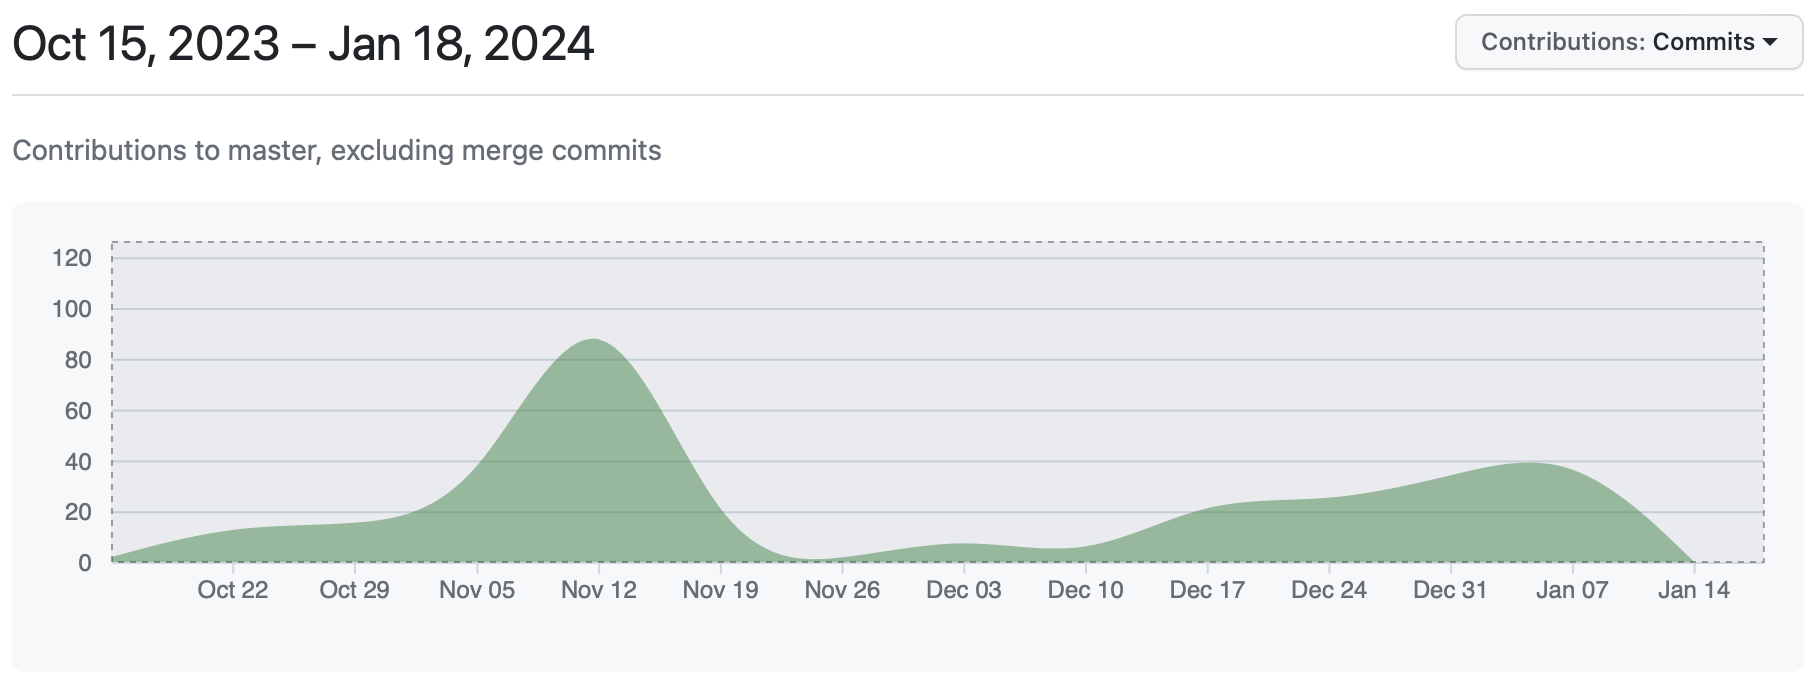
\includegraphics[scale=0.45]{dijagrami/d_pregleda1.png}%veličina slike u odnosu na originalnu datoteku i pozicija slike
			\centering
			\label{fig:promjene}
		\end{figure}
		 \begin{figure}[H]
			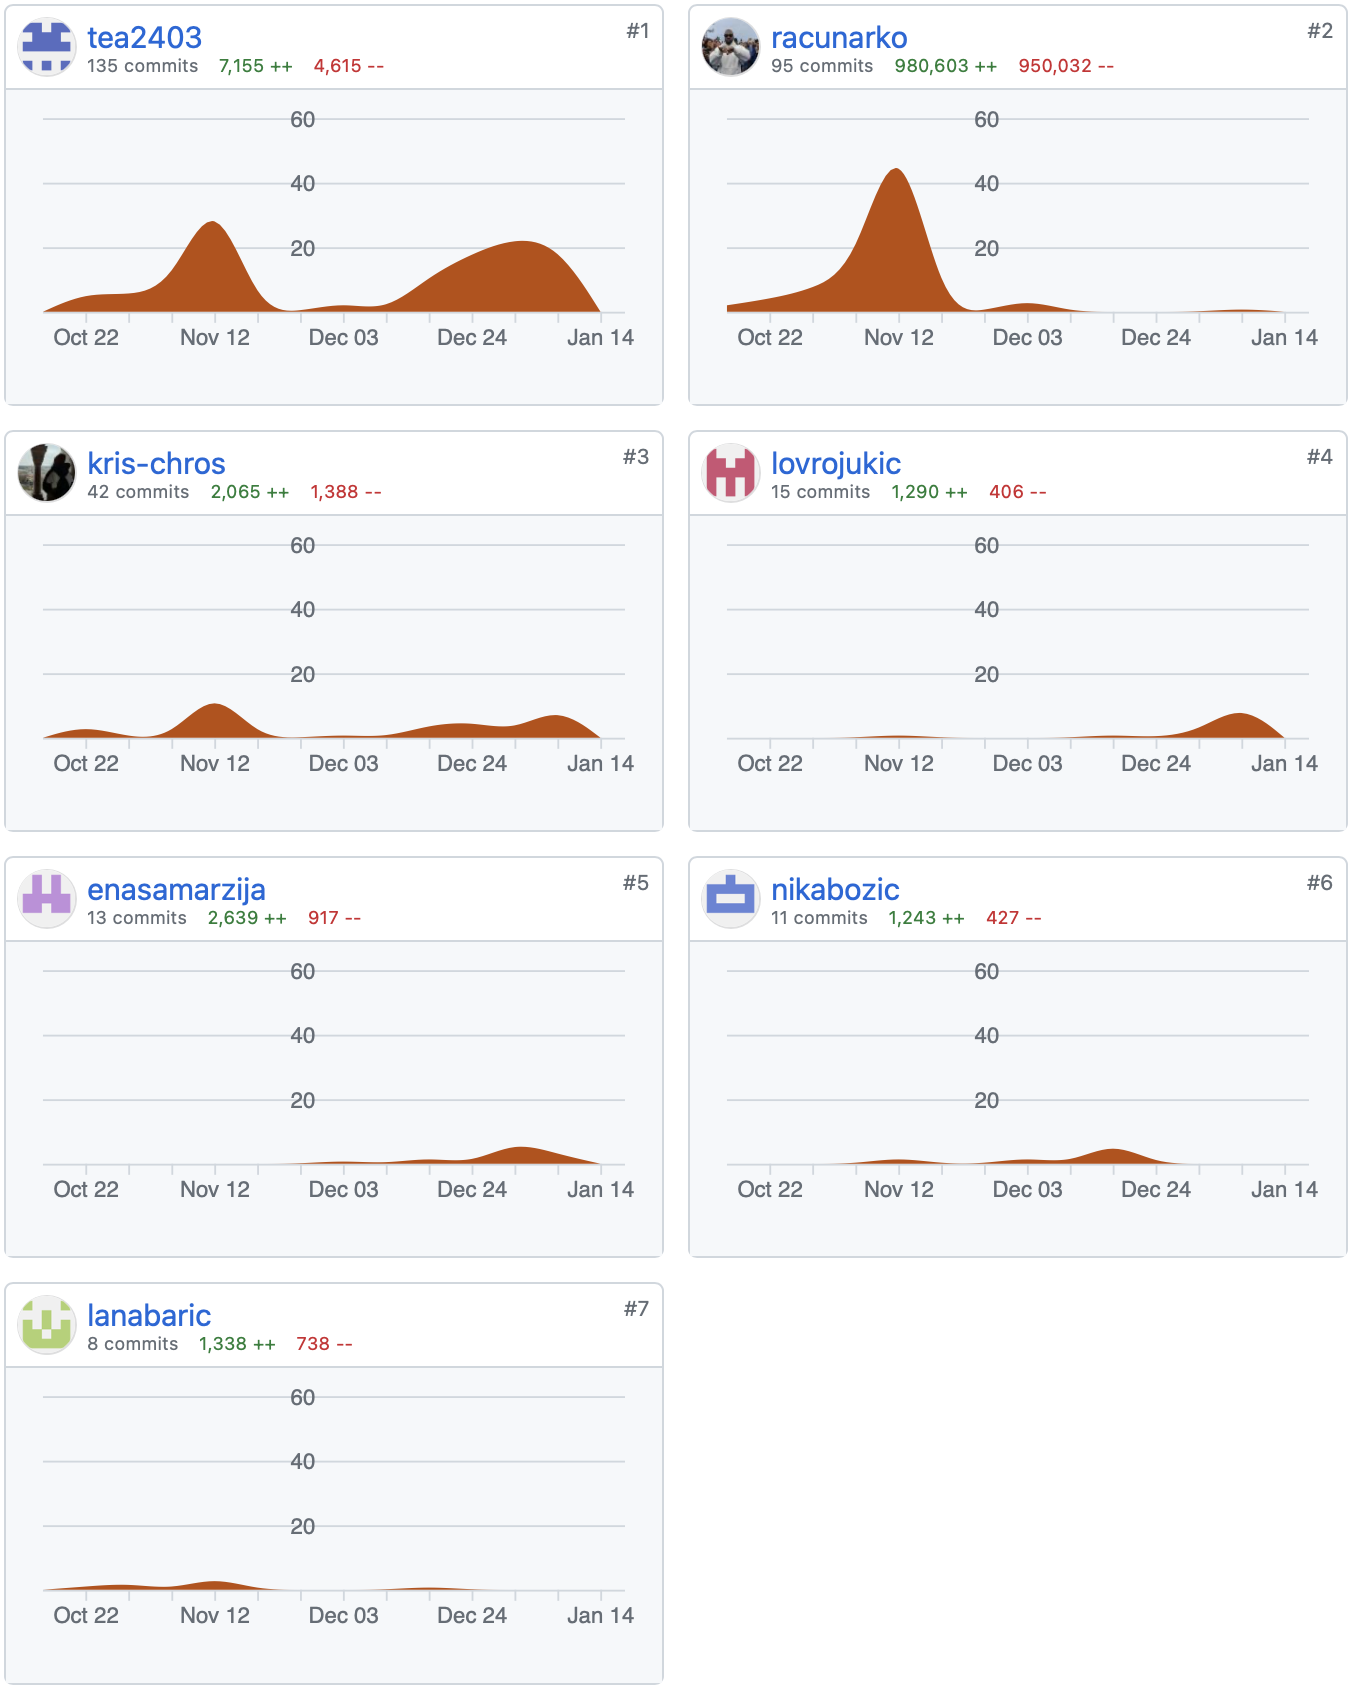
\includegraphics[scale=0.45]{dijagrami/d_pregleda2.png}%veličina slike u odnosu na originalnu datoteku i pozicija slike
			\centering
			\label{fig:promjene}
		\end{figure}
		
	